\subsection{MSVC: x86}

\RU{Вот что выходит на ассемблере}\EN{Here is what we get in the assembly output} (MSVC 2010):

\lstinputlisting{patterns/04_scanf/3_checking_retval/ex3_MSVC_x86.asm}

\index{x86!\Registers!EAX}
\RU{Для того чтобы вызывающая функция имела доступ к результату вызываемой функции, 
вызываемая функция (в нашем случае \scanf) оставляет это значение в регистре \EAX.}
\EN{The \Gls{caller} function (\main) needs the \gls{callee} function (\scanf) result, 
so the \gls{callee} returns it in the \EAX register.}

\index{x86!\Instructions!CMP}
\RU{Мы проверяем его инструкцией \TT{CMP EAX, 1} (\IT{CoMPare}), то есть 
сравниваем значение в \EAX с 1.}
\EN{We check it with the help of the instruction \TT{CMP EAX, 1} (\IT{CoMPare}).
In other words, we compare the value in the \EAX register with 1.} 

\index{x86!\Instructions!JNE}
\RU{Следующий за инструкцией \CMP: условный переход \JNE. 
Это означает \IT{Jump if Not Equal}, то есть условный переход \IT{если не равно}.}
\EN{A \JNE conditional jump follows the \CMP instruction. \JNE stands for \IT{Jump if Not Equal}.}

\RU{Итак, если \EAX не равен 1, то \JNE заставит \ac{CPU} перейти 
по адресу указанном в операнде \JNE, у нас это \TT{\$LN2@main}.}
\EN{So, if the value in the \EAX register is not equal to 1, 
the \ac{CPU} will pass the execution to the 
address mentioned in the \JNE operand, in our case \TT{\$LN2@main}.}
\RU{Передав управление по этому адресу, \ac{CPU} начнет исполнять вызов \printf с 
аргументом \TT{What you entered? Huh?}.}
\EN{Passing the control to this address results in the \ac{CPU} executing \printf 
with the argument \TT{What you entered? Huh?}.}
\RU{Но если всё нормально, перехода не случится и исполнится другой \printf с двумя аргументами: 
\TT{'You entered \%d...'} и значением переменной \TT{x}.}
\EN{But if everything is fine, the conditional jump is not be be taken, and another \printf call 
is to be executed, with two arguments: \TT{'You entered \%d...'} and the value of \TT{x}. }

\index{x86!\Instructions!XOR}
\index{\CLanguageElements!return}
\RU{Для того чтобы после этого вызова не исполнился сразу второй вызов \printf, 
после него есть инструкция \JMP, безусловный переход, который отправит процессор на место 
после второго \printf и перед инструкцией \TT{XOR EAX, EAX}, которая реализует \TT{return 0}.}
\EN{Since in this case the second \printf has not to be executed, there is a \JMP preceding it (unconditional jump). 
It passes the control to the point after the second \printf and just before the \TT{XOR EAX, EAX} instruction, which implements \TT{return 0}.}

\index{x86!\Registers!\Flags}
\RU{Итак, можно сказать что в подавляющих случаях сравнение какой-либо переменной с чем-то другим 
происходит при помощи пары инструкций \CMP и \Jcc, где \IT{cc} это \IT{condition code}.}
\EN{So, it could be said that comparing a value with another is \IT{usually} implemented
by \CMP/\Jcc instruction pair, where \IT{cc} is \IT{condition code}.}
\RU{\CMP сравнивает два значения и выставляет 
флаги процессора\footnote{См. также о флагах x86-процессора: \href{http://go.yurichev.com/17120}{wikipedia}.}.}
\EN{\CMP compares two values and sets 
processor flags\footnote{x86 flags, see also: \href{http://go.yurichev.com/17120}{wikipedia}.}.}
\RU{\Jcc проверяет нужные ему флаги и выполняет переход по указанному адресу (или не выполняет).}
\EN{\Jcc checks those flags and decides to either pass the control to the specified address or not.}

\index{x86!\Instructions!CMP}
\index{x86!\Instructions!SUB}
\label{CMPandSUB}
\RU{Но на самом деле, как это не парадоксально поначалу звучит, \CMP это почти то же самое что и 
инструкция \SUB, которая отнимает числа одно от другого.}
\EN{This could sound paradoxical, but the \CMP instruction is in fact \SUB (subtract).}
\RU{Все арифметические инструкции также выставляют флаги в соответствии с результатом, не только \CMP.}
\EN{All arithmetic instructions set processor flags, not just \CMP.}
\RU{Если мы сравним 1 и 1, от единицы отнимется единица, получится 0, и выставится флаг 
\ZF (\IT{zero flag}), означающий, что последний полученный результат был 0.}
\EN{If we compare 1 and 1, $1-1$ is 0 so the \ZF flag would be set (meaning that the last result was 0).}
\RU{Ни при каких других значениях \EAX, флаг \ZF не может быть выставлен, кроме тех, когда операнды равны друг другу.}
\EN{In no other circumstances \ZF can be set, except when the operands are equal.}
\index{x86!\Instructions!JNE}
\index{x86!\Registers!ZF}
\RU{Инструкция \JNE проверяет только флаг \ZF, и совершает переход только если флаг не поднят. 
Фактически, \JNE это синоним инструкции \JNZ (\IT{Jump if Not Zero}).}
\EN{\JNE checks only the \ZF flag and jumps only if it is not set. 
\JNE is in fact a synonym for \JNZ (\IT{Jump if Not Zero}).}
\RU{Ассемблер транслирует обе инструкции в один и тот же опкод.}
\EN{Assembler translates both \JNE and \JNZ instructions into the same opcode.}
\RU{Таким образом, можно \CMP заменить на \SUB и всё будет работать также, но разница в том, что \SUB 
всё-таки испортит значение в первом операнде. \CMP это \IT{SUB без сохранения результата, но изменяющая флаги}.}
\EN{So, the \CMP instruction can be replaced with a \SUB instruction 
and almost everything will be fine,
with the difference that \SUB alters the value of the first operand.
\CMP is \IT{SUB without saving the result, but affecting flags}.}

\ifx\LITE\undefined
\subsection{MSVC: x86: IDA}

\index{IDA}
\RU{Наверное, уже пора делать первые попытки анализа кода в \IDA}%
\EN{It is time to run \IDA and try to do something in it}.
\RU{Кстати, начинающим полезно компилировать в MSVC с ключом \TT{/MD}, что означает что все эти стандартные
функции не будут скомпонованы с исполняемым файлом, а будут импортироваться из файла \TT{MSVCR*.DLL}.}
\EN{By the way, for beginners it is good idea to use \TT{/MD} option in MSVC, which means that all these
standard functions are not be linked with the executable file, 
but are to be imported from the \TT{MSVCR*.DLL} file instead.}
\RU{Так будет легче увидеть, где какая стандартная функция используется.}
\EN{Thus it will be easier to see which standard function are used and where.}

\RU{Анализируя код в \IDA, очень полезно делать пометки для себя (и других).}
\EN{While analysing code in \IDA, it is very helpful to leave notes for oneself (and others)}.
\RU{Например, разбирая этот пример, мы сразу видим, что \TT{JNZ} срабатывает в случае ошибки.}
\EN{In instance, analysing this example, 
we see that \TT{JNZ} is to be triggered in case of an error.}
\RU{Можно навести курсор на эту метку, нажать \q{n} и переименовать метку в \q{error}.}
\EN{So it is possible to move the cursor to the label, press \q{n} and rename it to \q{error}.}
\RU{Ещё одну метку}\EN{Create another label}\EMDASH{}\RU{в}\EN{into} \q{exit}.
\RU{Вот как у меня получилось в итоге}\EN{Here is my result}:

\lstinputlisting{patterns/04_scanf/3_checking_retval/ex3.lst}

\RU{Так понимать код становится чуть легче}\EN{Now it is slightly easier to understand the code}.
\RU{Впрочем, меру нужно знать во всем и комментировать каждую инструкцию не стоит.}
\EN{However, it is not a good idea to comment on every instruction.}

% FIXME draw button?
\RU{В \IDA также можно скрывать части функций: нужно выделить скрываемую часть, нажать \q{--} на цифровой клавиатуре и ввести текст}
\EN{You could also hide(collapse) parts of a function in \IDA.
To do that mark the block, then press \q{--} on the numerical pad and enter the text to be displayed instead}.

\RU{Я скрыл две части и придумал им названия}\EN{I have hidden two blocks and given them names}:

\lstinputlisting{patterns/04_scanf/3_checking_retval/ex3_2.lst}

% FIXME draw button?
\RU{Раскрывать скрытые части функций можно при помощи \q{+} на цифровой клавиатуре}
\EN{To expand previously collapsed parts of the code, use \q{+} on the numerical pad}.

\clearpage
\RU{Нажав \q{пробел}, мы увидим, как \IDA может представить функцию в виде графа}\EN{By pressing \q{space},
we can see how \IDA represents a function as a graph}:

\begin{figure}[H]
\centering
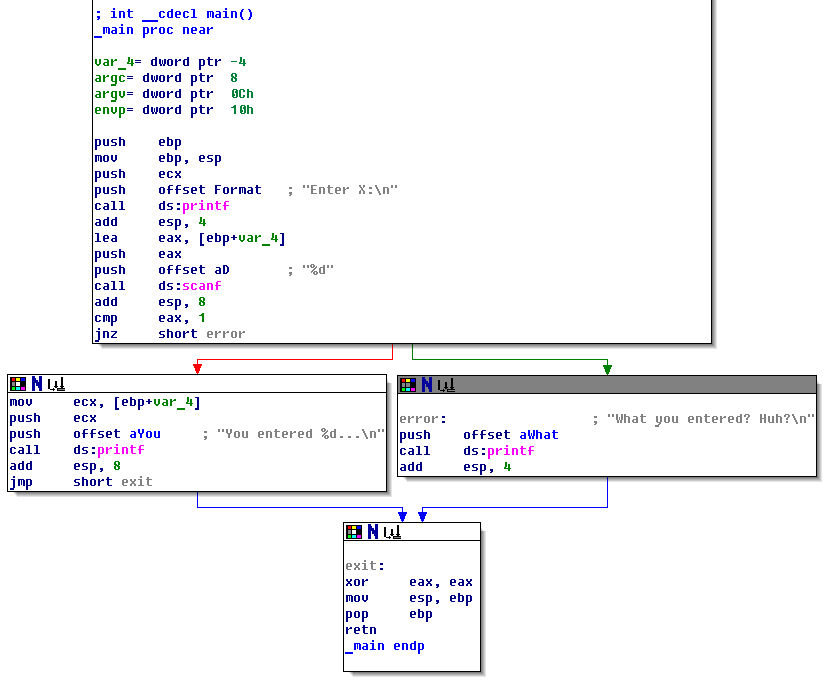
\includegraphics[scale=\FigScale]{patterns/04_scanf/3_checking_retval/IDA.png}
\caption{\RU{Отображение функции в IDA в виде графа}\EN{Graph mode in IDA}}
\label{fig:ex3_IDA_1}
\end{figure}

\RU{После каждого условного перехода видны две стрелки: зеленая и красная}\EN{There are two arrows
after each conditional jump: green and red}.
\RU{Зеленая ведет к тому блоку, который исполнится если переход сработает, 
а красная~--- если не сработает.}
\EN{The green arrow points to the block which executes if the jump is triggered, 
and red if otherwise.}

\clearpage
\RU{В этом режиме также можно сворачивать узлы и давать им названия}
\EN{It is possible to fold nodes in this mode and give them names as well} (\q{group nodes}).
\RU{Я сделал это для трех блоков}\EN{I did it for 3 blocks}:

\begin{figure}[H]
\centering
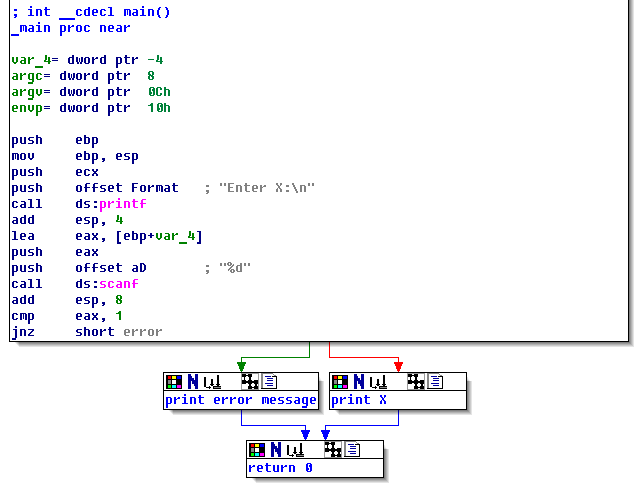
\includegraphics[scale=\FigScale]{patterns/04_scanf/3_checking_retval/IDA2.png}
\caption{\RU{Отображение в IDA в виде графа с тремя свернутыми блоками}\EN{Graph mode in IDA with 3 nodes folded}}
\label{fig:ex3_IDA_2}
\end{figure}

\RU{Всё это очень полезно делать}\EN{That is very useful}.
\RU{Вообще, очень важная часть работы реверсера состоит в том, чтобы уменьшать количество имеющейся информации.}
\EN{It could be said that a very important part of the reverse engineers' job is to reduce the amount of information they deal with.}
\fi

\ifdefined\IncludeOlly
\clearpage
\subsection{MSVC: x86 + \olly}

\RU{Попробуем в \olly немного хакнуть программу и сделать вид, что \scanf срабатывает всегда без ошибок.}
\EN{Let's try to hack our program in \olly, forcing it to think \scanf always works without error.}

\RU{Когда в \scanf передается адрес локальной переменной, изначально в этой переменной
находится некий мусор. В данном случае это}\EN{When an address of a local variable is passed into \scanf,
the variable initially contains some random garbage, in this case} \TT{0x6E494714}:

\begin{figure}[H]
\centering
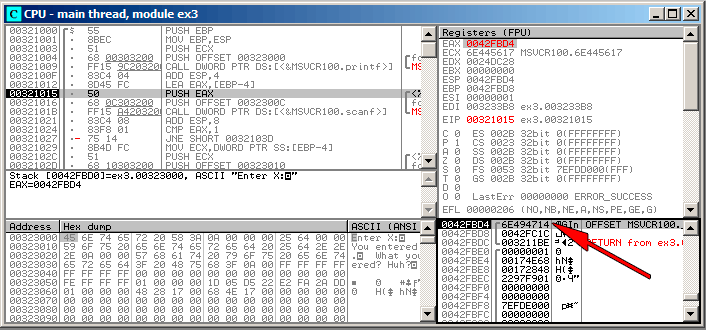
\includegraphics[scale=\FigScale]{patterns/04_scanf/3_checking_retval/olly_1.png}
\caption{\olly: \RU{передача адреса переменной в}\EN{passing variable address into} \scanf}
\label{fig:scanf_ex3_olly_1}
\end{figure}

\clearpage
\RU{Когда}\EN{While} \scanf \RU{запускается, я ввожу в консоли что-то непохожее на число, например}
\EN{executes, in the console I enter something that is definitely not a number, like} ``asdasd''.
\scanf \RU{заканчивается с 0 в}\EN{finishes with 0 in} \EAX, \RU{что означает, что произошла ошибка}%
\EN{which indicates that an error has occurred}:

\begin{figure}[H]
\centering
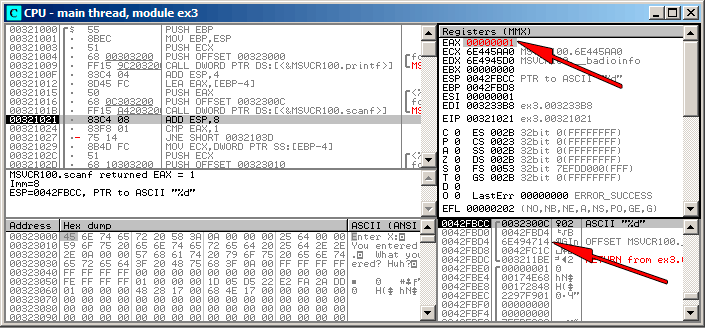
\includegraphics[scale=\FigScale]{patterns/04_scanf/3_checking_retval/olly_2.png}
\caption{\olly: \scanf \RU{закончился с ошибкой}\EN{returning error}}
\label{fig:scanf_ex3_olly_2}
\end{figure}

\RU{Вместе с этим мы можем посмотреть на локальную переменную в стеке~--- она не изменилась.}
\EN{We can also check the local variable in the stack and note that it has not changed.}
\RU{Действительно, ведь что туда записала бы функция \scanf}\EN{Indeed, what would \scanf write there}?
\RU{Она не делала ничего кроме возвращения нуля}\EN{It simply did nothing except returning zero}.

\RU{Попробуем ещё немного ``хакнуть'' нашу программу}\EN{Let's try to ``hack'' our program}.
\RU{Щелкнем правой кнопкой на}\EN{Right-click on} \EAX, \RU{там, в числе опций, будет также}
\EN{Among the options there is} ``Set to 1''.
\RU{Это нам и нужно}\EN{This is what we need}.

\RU{В \EAX теперь 1, последующая проверка пройдет как надо, и \printf выведет значение переменной
из стека.}
\EN{We now have 1 in \EAX, so the following check is to be executed as intended, 
and \printf will print the value of the variable in the stack.}

\RU{Запускаем (F9) и видим в консоли следующее:}
\EN{When we run the program (F9) we can see the following in the console window:}

\begin{figure}[H]
\centering
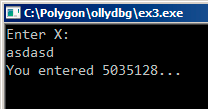
\includegraphics[scale=\FigScale]{patterns/04_scanf/3_checking_retval/olly_3.png}
\caption{\RU{консоль}\EN{console window}}
\end{figure}

\RU{Действительно}\EN{Indeed}, $1850296084$ \RU{это десятичное представление числа в стеке}
\EN{is a decimal representation of the number in the stack} (\TT{0x6E494714})!

\fi

\clearpage
\subsection{MSVC: x86 + Hiew}
\index{Hiew}

\RU{Это ещё может быть и простым примером исправления исполняемого файла}\EN{This can also be used as 
a simple example of executable file patching}.
\RU{Мы можем попробовать исправить его таким образом, что программа всегда будет выводить числа,
вне зависимости от ввода}\EN{We may try to patch the executable so the program would always 
print the input, no matter what we enter}.

\RU{Исполняемый файл скомпилирован с импортированием функций из}\EN{Assuming that the 
executable is compiled against external} \TT{MSVCR*.DLL} (\RU{т.е. с опцией}\EN{i.e., with} 
\TT{/MD}\EN{ option})\footnote{\RU{то, что ещё называют}\EN{that's what also called} \q{dynamic linking}}, 
\RU{поэтому мы можем отыскать функцию}\EN{we see the} \main \RU{в самом начале секции}\EN{function at the 
beginning of the} \TT{.text}\EN{ section}.
\RU{Откроем исполняемый файл в Hiew, найдем самое начало секции}\EN{Let's open the executable in Hiew and 
find the beginning of the} \TT{.text}\EN{ section} (Enter, F8, F6, Enter, Enter).

\RU{Мы увидим следующее}\EN{We can see this}:

\begin{figure}[H]
\centering
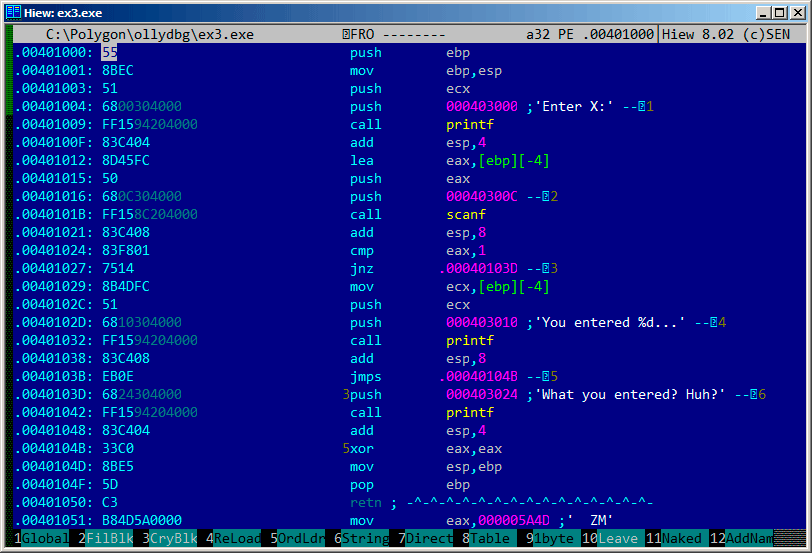
\includegraphics[scale=\FigScale]{patterns/04_scanf/3_checking_retval/hiew_1.png}
\caption{Hiew: \RU{функция }\main\EN{ function}}
\label{fig:scanf_ex3_hiew_1}
\end{figure}

Hiew \RU{находит}\EN{finds} \ac{ASCIIZ}\RU{-строки и показывает их, также как и имена импортируемых 
функций}\EN{ strings and displays them, as it does with the imported functions' names}.

\clearpage
\RU{Переведите курсор на адрес}\EN{Move the cursor to address} \TT{.00401027} 
(\RU{с инструкцией}\EN{where the} \TT{JNZ}\RU{, которую мы хотим заблокировать}\EN{ instruction, we 
have to bypass, is located}), \RU{нажмите}\EN{press} F3,
\RU{затем наберите}\EN{and then type} \q{9090}(\RU{ что означает два}\EN{, meaning two} \ac{NOP}\RU{-а}\EN{s}): 

\begin{figure}[H]
\centering
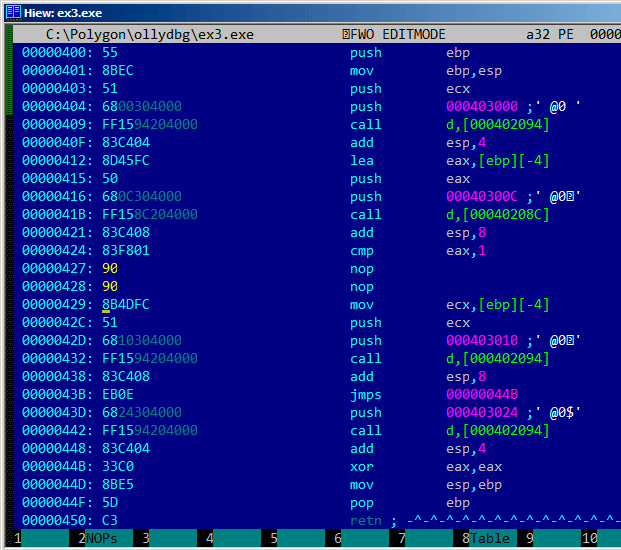
\includegraphics[scale=\FigScale]{patterns/04_scanf/3_checking_retval/hiew_2.png}
\caption{Hiew: \RU{замена}\EN{replacing} \TT{JNZ} \RU{на два}\EN{with two} \ac{NOP}\RU{-а}\EN{s}}
\label{fig:scanf_ex3_hiew_2}
\end{figure}

\RU{Затем}\EN{Then press} F9 (update). \RU{Теперь исполняемый файл записан на диск. Он будет вести себя
так, как нам надо.}\EN{Now the executable is saved to the disk. It will behave as we wanted.}

\RU{Два}\EN{Two} \ac{NOP}\RU{-а}\EN{s} \RU{возможно, не так эстетично, как могло бы быть}\EN{are probably 
not the most \ae{}sthetic approach}.
\RU{Другой способ изменить инструкцию это записать 0 во второй байт опкода (смещение перехода),
так что}\EN{Another way to patch this instruction is to write just 0 to the second opcode byte (\gls{jump offset}), 
so that} \TT{JNZ} \RU{всегда будет переходить на следующую инструкцию}\EN{will always jump to 
the next instruction}.

\RU{Можно изменить и наоборот: первый байт заменить на \TT{EB}, второй байт (смещение перехода) не трогать.}
\EN{We could also do the opposite: replace first byte with \TT{EB} while not touching the second byte (\gls{jump offset}).}
\RU{Получится всегда срабатывающий безусловный переход}\EN{We would get an unconditional jump that is always triggered}.
\RU{Теперь сообщение об ошибке будет выдаваться всегда, даже если мы ввели число.}
\EN{In this case the error message would be printed every time, no matter the input.}
